\documentclass[usenames,dvipsnames]{beamer}
\usetheme{Berlin}
\usepackage[utf8]{inputenc}
\usepackage[english]{babel}
\usepackage{graphicx}
\usepackage{url}
\usepackage{multicol}
\usepackage{relsize}
\usepackage{enumitem}
\usepackage{fancyvrb}

\graphicspath{ {images/} }

\title{Secure memory handling in C}
\subtitle{}
\author{Alexander Livenets \\ Oliver Esser}
\institute{}
\date{25 June 2019}

\newcommand{\codeinline}[1] {\texttt{\smaller[2]{#1}}}
\newcommand{\greenalert}[1] {\alert{\textcolor{green}{#1}}}
\newcommand{\redalert}[1] {\alert{\textcolor{red}{#1}}}
\begin{document}

\AtBeginSection[]
{
\begin{frame}
\frametitle{Table of Contents}
\tableofcontents[currentsection]
\end{frame}
}

\setbeamertemplate{endpage}{%
\begin{frame}
\center \Huge Thanks!
\end{frame}
}

\begin{frame}
\titlepage
\end{frame}

\section{Memory handling}
\begin{frame}[fragile]
\frametitle{Buffer overflow example}
\tiny
\begin{columns}
\begin{column}{0.5\textwidth}
\begin{semiverbatim}
\uncover<1->{int copy\_string(const char *s) \{}
\uncover<1->{char buffer[16];}
\uncover<1->{  strcpy(buffer, s);}
\uncover<1->{\}}
\uncover<1->{}
\uncover<1->{int main(void) \{}
\uncover<1->{  char large\_string[128] = "Hello World!";}
\uncover<1->{  \alert<2->{\only<2->{\color{green}}copy\_string(large\_string);} \visible<2->{\only<2->{\color{green} \textbf{//OK...}}}}
\uncover<1->{\color{black}}
\uncover<1->{  // Fill large string}
\uncover<1->{  for(int i = 0; i < sizeof(large\_string)-1; ++i) \{}
\uncover<1->{    large\_string[i] = 'a';}
\uncover<1->{    large\_string[sizeof(large\_string)-1] = '\\0';}
\uncover<1->{  \}}
\uncover<1->{  \alert<3->{copy\_string(large\_string);} \visible<3->{\alert{\textbf{// Overflow...}}} }
\uncover<1->{\}}
\end{semiverbatim}
\end{column}
\pause
\begin{column}<4->{0.5\textwidth}
\begin{semiverbatim}
ASM (IA32):
 
main:
  ...
  mov [&large_string], \%ebx
  call [copy_string] // push \%eip on stack and jump

copy_string:
  push \%ebp
  mov \%esp, \%ebp
  push \%ebx
  leal -20(\%ebp), \%ebx // store  `&str` in register
  call [strcpy] // call `strcpy(str)`
  leave // restore stack frame
  ret // restore \%eip

\end{semiverbatim}

\end{column}
\end{columns}
\note{When string on stack overflows, return address or other sensitive data on stack may be corrupted, hence allowing to perform attack}
\end{frame}

\begin{frame}
\centering
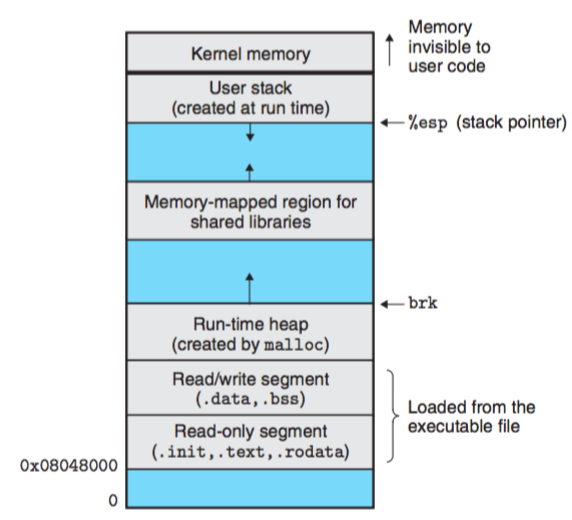
\includegraphics[scale=0.35]{linux_mem.png}

\tiny{\url{https://people.cs.pitt.edu/~xianeizhang/notes/Linking.html}}
\end{frame}

\begin{frame}
\centering
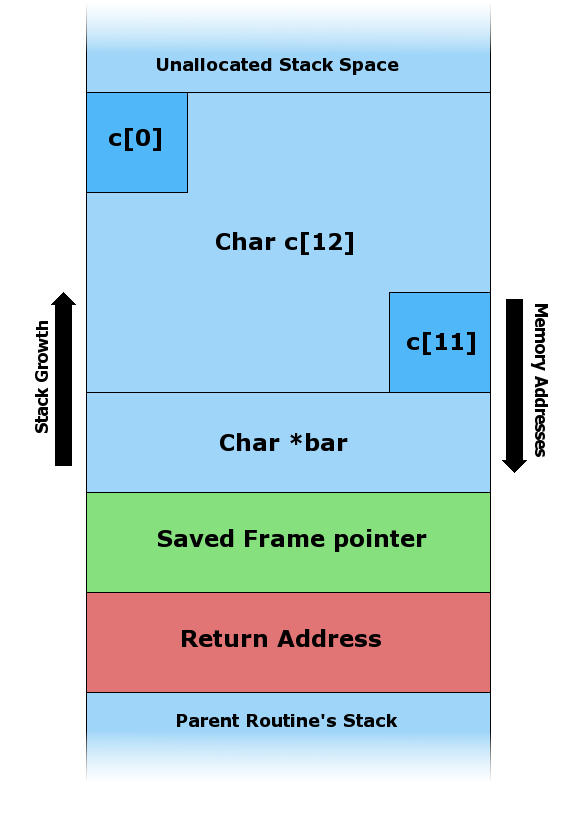
\includegraphics[scale=0.16]{Stack_Overflow_2.png}
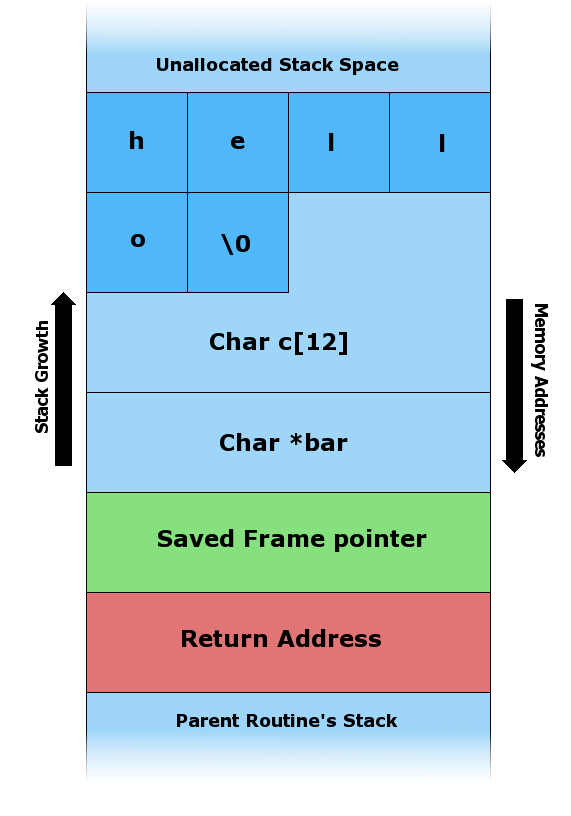
\includegraphics[scale=0.16]{Stack_Overflow_3.png}
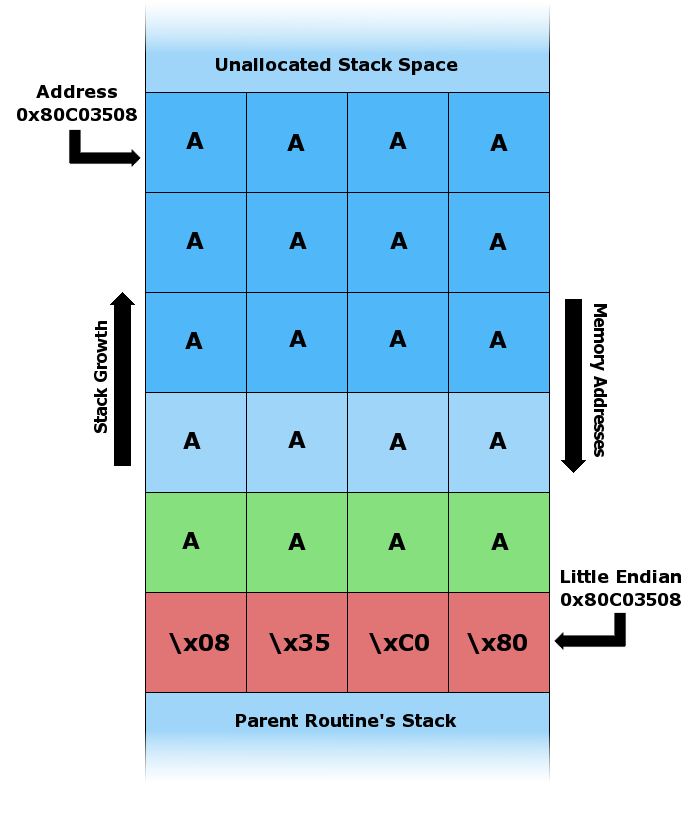
\includegraphics[scale=0.16]{Stack_Overflow_4.png}

\tiny{\url{https://en.wikipedia.org/wiki/Stack_buffer_overflow}}

\note{Show results of buffer overflow: return address may be overwritten and function will return to the malicious address}
\note{The same thing is with heap overflow}
\end{frame}

\section{libc}
\subsection{strcpy family}
\begin{frame}[fragile]
\frametitle{strcpy, strcat}
\begin{itemize}[label={},leftmargin=*]
\item \codeinline{char *strcpy(char *dst, const char *src);}
\item \codeinline{char *strncpy(char *dst, const char *src, size\_t dst\_size);}
\item \codeinline{char *strcat(char *dst, const char *src);}
\item \codeinline{char *strncat(char *dst, const char *src, size\_t dst\_size);}
\end{itemize}

\par
\codeinline{man strcpy, BUGS section:}
\tiny
\begin{semiverbatim}
If the \alert{\textbf{destination string of a strcpy() is not large enough, then anything might happen}}.
Overflowing fixed-length string buffers is a favorite cracker technique for taking complete
control of the machine. Any time a program reads or copies data into a buffer, the program
first needs to check that there's enough space. This may be unnecessary if you can show that
overflow is impossible, but be careful: \alert{\textbf{programs can get changed over time,
in ways that may make the impossible possible.}}
\end{semiverbatim}
\end{frame}

\begin{frame}[fragile]
\frametitle{strcpy, strcat}
\small
\begin{verbatim}
char src[32] = "HELLO";
char src2[] = "WORLD"
char dest[16] = {0};

strncpy(dest, src, sizeof(dest));

strncat(dest, src, sizeof(dest));
strncat(dest + strlen(dest), src2, sizeof(dest) - strlen(dest));
\end{verbatim}
\end{frame}

\subsection{sprintf family}
\begin{frame}[fragile]
\frametitle{sprintf, snprintf}
\begin{itemize}[label={},leftmargin=*]
\item \codeinline{int sprintf(char *str, char *fmt, ...);}
\item \codeinline{int snprintf(char *str, size\_t len, char *fmt, ...);}
\end{itemize}
\end{frame}

\begin{frame}[fragile]
\frametitle{sprintf, snprintf}
\small
\begin{verbatim}
char src[32] = "HELLO";
char src2[] = "WORLD"
char dest[16] = {0};

int count;

count = sprintf(dest, "%s", src);

count = snprintf(dest, sizeof(dest), "%s", src);
count = snprintf(dest + count - 1, sizeof(dest) - count + 1, "%s", src2);
\end{verbatim}
\end{frame}

\section{libbsd}
\subsection{strlcpy, strlcat}
\begin{frame}[fragile]
\frametitle{strlcpy, strlcat}
\codeinline{libbsd:}
\begin{itemize}[label={},leftmargin=*]
\item \codeinline{size\_t strlcpy(char *dst, const char *src, size\_t dst\_size);}
\item \codeinline{size\_t strlcat(char *dst, const char *src, size\_t dst\_size);}
\end{itemize}
\end{frame}

\begin{frame}[fragile]
\frametitle{strlcpy, strlcat}
\tiny
\begin{verbatim}
char src[32] = "HELLO";
char src2[] = "WORLD"
char dest[16] = {0};
int count;

count = strlcpy(dest, src, sizeof(buf));
if (count >= sizeof(dest))
  handle_truncation_condition();

dest[0] = '\0';
count = strlcat(dest, src, sizeof(dest));
if (count >= sizeof(dest))
  handle_truncation_condition();

count = strlcat(dest, src2, sizeof(dest));
if (count >= sizeof(dest))
  handle_truncation_condition();
\end{verbatim}
\end{frame}

\section{Good practices}
\subsection{Refactoring}

\begin{frame}[fragile]
\frametitle{Code}
\tiny
\begin{semiverbatim}
\#include <cstdio>
\#include <cstring>

int copy\_string(char *dest, const char *src) \{
  // Magic copy 
  \redalert{strcpy(dest, src);}
\}

int main(int argc, char *argv[]) \{ 
  char buffer[16];

  if (argc < 2) \{
    printf("Usage: \%s STRING\\n", argv[0]);
    return 0;
  \}

  \redalert{copy\_string(buffer, argv[1]);}
  printf("Copied string, contents of the buffer:\\n\%s", buffer);

  return 0;
\}
\end{semiverbatim}
\end{frame}

\begin{frame}[fragile]
\frametitle{C: Example 1}
\tiny
\begin{semiverbatim}
\#include <cstdio>
\#include <cstring>

int copy\_string(char *dest, const char *src, size\_t len) \{
  // Magic copy
  \greenalert{strncpy(dest, src, len);}
\}

int main(int argc, char *argv[]) \{
  char buffer[16];

  if (argc < 2) \{
    printf("Usage: \%s STRING\\n", argv[0]);
    return 0;
  \}

  \greenalert{copy\_string(buffer, argv[1], sizeof(buffer));}
  printf("Copied string, contents of the buffer:\\n\%s", buffer);

  return 0;
\}
\end{semiverbatim}
\end{frame}

\begin{frame}
\frametitle{C: Example 2}
\tiny
\begin{semiverbatim}
\#include <cstdio>
\#include <cstring>

\greenalert{int copy\_string(char *dest, const char *src, size\_t len) \{} 
  \\ // Magic copy \\
  \greenalert{strncpy(dest, src, len - 1);}
  if (len > 0)
    dest[len - 1] = '\\0';
\}

int main(int argc, char *argv[]) \{
  char buffer[16];

  if (argc < 2) \{
    printf("Usage: \%s STRING\\n", argv[0]);
    return 0;
  \}

  \greenalert{copy\_string(buffer, argv[1], sizeof(buffer));}
  printf("Copied string, contents of the buffer:\\n\%s", buffer);

  return 0;
\}
\end{semiverbatim}
\end{frame}

\begin{frame}
\frametitle{C: Example 3}
\tiny
\begin{semiverbatim}
\#include <cstdio>
\#include <cstring>

\greenalert{int copy\_string(char *dest, const char *src, size\_t len) \{} 
  \\ // Magic print \\
  \greenalert{return snprintf(dest, len, "\%s", src);}
\}

int main(int argc, char *argv[]) \{
  char buffer[16];

  if (argc < 2) \{
    printf("Usage: \%s STRING\\n", argv[0]);
    return 0;
  \}

  \greenalert{copy\_string(buffer, argv[1], sizeof(buffer));}
  printf("Copied string, contents of the buffer:\\n\%s", buffer);

  return 0;
\}
\end{semiverbatim}
\end{frame}

\begin{frame}[fragile]
\frametitle{C++: Example 3}
\tiny
\begin{semiverbatim}
\#include <array>
\#include <cstdio>
\#include <cstring>

template <size\_t N>
\greenalert{int copy\_string(std::array<char, N> &dest, const char *src) \{}
  // Magic copy 
  strncpy(&dest[0], src, N - 1);
  if (N > 0)
    dest[N - 1] = '\\0';
\}

int main(int argc, char *argv[]) \{
  \greenalert{std::array<char, 16> buffer;}

  if (argc < 2) \{
    printf("Usage: \%s STRING\\n", argv[0]);
    return 0;
  \}

  \greenalert{copy\_string(buffer, argv[1]);}
  printf("Copied string, contents of the buffer:\\n\%s", &buffer[0]);

  return 0;
\}
\end{semiverbatim}
\end{frame}

\begin{frame}
\frametitle{C++: Example 4}
\tiny
\begin{semiverbatim}
\#include <array>
\#include <algorithm>
\#include <cstdio>
\#include <cstring>

template <size\_t N>
\greenalert{int copy\_string(std::array<char, N> \&dest, std::string\_view src) \{}
  \greenalert{std::copy\_n(src.begin(), N, dest.begin());}
  if (N > 0)
    dest[N - 1] = '\\0';
\}

int main(int argc, char *argv[]) \{
  std::array<char, 16> buffer;

  if (argc < 2) \{
    printf("Usage: \%s STRING\\n", argv[0]);
    return 0;
  \}

  \greenalert{copy\_string(buffer, argv[1]);}
  printf("Copied string, contents of the buffer:\\n\%s", \&buffer[0]);

  return 0;
\}
\end{semiverbatim}
\end{frame}

\subsection{Compiler tricks and tips}
\begin{frame}
\frametitle{\subsecname}
\small
GCC compiler parameters:
\begin{itemize}[leftmargin=*]
	\setlength\itemsep{0.3em}
	\item \codeinline{-Wformat=\{1,2\} -Wformat-nonliteral -Wformat-overflow -Wformat-signedness -Wformat-y2k -Wformat-security -Wformat-nonliteral} \\
	\visible<2->{Ex.: \codeinline{int my\_printf(struct MyContext *ctx, const char *fmt, ....) \_\_attribute\_\_((format (printf, 2, 3)));}}
	\item \codeinline{-Wformat-truncation=\{1,2\}}
	\item \codeinline{-Wstringop-overflow=\{1,2,3,4\}}
	\item \codeinline{-Wstringop-truncation}
	\item \codeinline{-Warray-bounds=\{1,2\}}
\end{itemize}

GCC instrumentation options:
\begin{itemize}[leftmargin=*]
	\setlength\itemsep{0.3em}
	\item \codeinline{-fstack-protector-\{all,strong,explicit,\}}
	\item \codeinline{-fsanitize=address}
	\item \codeinline{-fsanitize=undefined -fsanitize=null -fsanitize=bounds -fsanitize=bounds-strict}
	\item \codeinline{-fsanitize=pointer-compare -fsanitize=pointer-subtract}
	\item \codeinline{-fsanitize=pointer-overflow}
	\item \codeinline{-fsanitize-address-use-after-scope}
\end{itemize}
\end{frame}

\subsection{Recommendations}
\begin{frame}
\frametitle{\subsecname}
\begin{itemize}[leftmargin=*]
	\item C: Use C \textgreater= C99(best, use C11), declaring \codeinline{snprintf}
	\item C: readings strings from input: DON'T USE \codeinline{scanf} with \codeinline{\%s} and \codeinline{gets}, use 
	\codeinline{fgets}
	\item C: Don't use strcpy and similar!!! use function accepting buffer size parameter: \codeinline{strn\*}: \codeinline{strncpy, strnlen,...}
	\item C: use libbsd with safer functions
	\item C APIs: write C++ API wrappers
	\item C++: use \codeinline{std::ostringstream}
	\item C++: \codeinline{std::string}, \codeinline{std::string\_view} (C++17), \codeinline{std::span} (C++20)
	\item When writing functions, pass max. buffer size in function, e.g.: \codeinline{void f(char *s, size\_t len);}
	\item Use \codeinline{snprintf} to copy strings
	\item Validate input data from external sources
	\item Common: Secure Coding Practices, Safe Coding Practices
\end{itemize}
\end{frame}

\section{References}
\begin{frame}
\frametitle{\secname}
\footnotesize
\begin{itemize}[leftmargin=*]
	\item \url{https://people.cs.pitt.edu/~xianeizhang/notes/Linking.html}
	\item \url{https://safecode.org/courses/secure-memory-handling-in-c-101/}
\end{itemize}
\end{frame}

\usebeamertemplate{endpage}

\end{document}
